%%% A Sample Clinic Report Written Using LaTeX.
%%%
%%% C.M. Connelly <cmc@math.hmc.edu>
%%%
%%%  $Id: sample-thesis-report.tex 171 2005-09-01 18:12:30Z cmc $

%%% Copyright (C) 2004-2005 Claire M. Connelly and 
%%% the Department of Mathematics, Harvey Mudd College.
%%%
%%% This file is part of the sample thesis document provided to HMC
%%% mathematics students.
%%%
%%% See the COPYING document, which should accompany this
%%% distribution, for information about distribution and modification
%%% of the document and its components.


%%% The top part of your document is called the preamble.  You supply
%%% some basic information about the document (such as its title and
%%% author) in a form that LaTeX can understand here.

%%% You can also load additional LaTeX packages, or style files, that
%%% affect the way that the document is laid out, typeset, or supply
%%% additional commands or environments.

%%% The preamble can also be used to define your own commands and
%%% environments, set some constants that will be used throughout your
%%% document, and so on.

%%% As you may have guessed, LaTeX's comment character is the percent
%%% sign.  Any line that starts with a % will be ignored.  You can
%%% also use the comment character to add comments to the end of a
%%% line that will be parsed by TeX.


%%% The first active line in your LaTeX document is the \documentclass
%%% command, which loads a LaTeX class file.  Class files generally
%%% define the appearance of a document, and include a variety of
%%% structural commands.

%%% Clinic reports use the clinic class, which should be located
%%% somewhere in TeX's search path.

%%% For midyear reports, include the midyear option, as in
\documentclass[mathematics,finalreport]{hmcclinic}

%%% Other packages needed by your document may be loaded here.
\usepackage{url}              % For formatting URLs and other web or
                              % file references.
\usepackage{mflogo}           % Provides the METAFONT logo.
\usepackage{booktabs}         % Publication-quality tables.
% \usepackage{natbib}           % Provides some nice citation and
                              % bibliography formatting commands.
% \bibpunct[:~]{(}{)}{;}{a}{,}{,~} % Set some defaults for bibliographic
                                 % punctuation used by natbib.sty.
% \bibliographystyle{abbrvnat}
\usepackage{apacite}
\usepackage{verbatim}
\usepackage{graphicx}
\usepackage{calc}
\usepackage{subfig}
\usepackage{textcomp}
\usepackage{float}
\usepackage[plainpages=false,pdfpagelabels]{hyperref}
\hypersetup{hidelinks,breaklinks=true,bookmarksopen=false,pdftitle={Title},pdfauthor={Author}}


\includeonly{%
%%% Chapter 1
introduction
%%% Chapter 2
,executive-summary
%%% Chapter 3
,automation
%%% Chapter 4
,topic-modeling
%%% Chapter 5
,conclusion
%%% Chapter 6
,future-work
%%% Chapter 7
,resources
%%% Chapter 8
,books
%%% Appendix
,versions
}


%%% Provide additional context around errors. 
\setcounter{errorcontextlines}{1000}

%%% Information about this document.

%%% I find it most useful to put identifying information about a
%%% document near the top of the preamble.  Technically, this
%%% information must precede the \maketitle command, which often
%%% appears immediately after the beginning of the document 
%%% environment.  Placing it near the top of the document makes it
%%% easier to identify the document, and keeps it out from getting
%%% mixed up with the real meat of the document.

%%% So, some questions.

%% What is the name of the company or organization sponsoring your project?
\sponsor{PilotCity}

%% What is the title of your report?
\title{Automating an Engine to Extract Educational Priorities for Workforce City Innovation}

%% Who are the authors of the report (your team members)?  (Separate
%% names with \and.)
\author{Madison Hobbs (Project Manager) \and Jean Selasi Adedze \and Dominique Macias \and
  Xuming Liang \and Aanya Alwani}

%% What is your faculty advisor's name?  (Again, separate names with
%% \and, if necessary.)
\advisor{Dr. Talithia Williams}

%% Liaison's name or names?
\liaison{Derick Lee, PilotCity}

%% Did you have an outside consultant help you with this project?  Put
%% their names in the \consultant command.
%% \consultant{Joseph Jones}

%%% End of information section.

%%% New commands and environments.

%%% You can define your own commands and environments here.  If you
%%% have a lot of material here, you might want to consider splitting
%%% the commands and environments into a separate ``style'' file that
%%% you load with \usepackage.

\newcommand{\coolcommand}[1]{#1 is cool.} % Lets everyone know that
                                % the person or thing that you provide
                                % as the argument to the command is
                                % cool.

%%% You probably won't want any of the following commands, which are
%%% here to allow various the names of commands, make examples typeset
%%% properly, and so on.  You can, of course, use them as examples for
%%% your own user-defined commands.
                                                                               
\newcommand{\bslash}{\symbol{'134}}%backslash
\newcommand{\bsl}{{\texttt{\bslash}}}
\newcommand{\com}[1]{\bsl\texttt{#1}\xspace}
\newcommand{\file}[1]{\texttt{#1}\xspace}

\newcommand{\pdftex}{PDF\tex}
\newcommand{\pdflatex}{PDF\latex}
\newcommand{\acronym}[1]{\textsc{#1}\xspace}
\newcommand{\key}[1]{\textsf{\emph{#1}}\xspace}
\newcommand{\class}[1]{\textsf{#1}\xspace}
\newcommand{\package}[1]{\textsf{#1}\xspace}
\newcommand{\env}[1]{\texttt{#1}\xspace}
\newcommand{\prog}[1]{\texttt{#1}\xspace}
\newcommand{\command}[1]{\texttt{\bsl{}#1}\xspace}
\newcommand{\ctt}{\texttt{comp.text.tex}\xspace}
\newcommand{\tex}{\TeX\xspace}
\newcommand{\latex}{\LaTeX\xspace}
\newcommand{\host}[1]{\textsf{#1}\xspace}
                                                                                


\newcounter{cms}

%%% Some theorem-like command definitions.

%%% The \newtheorem command comes from the amsthm package.  That
%%% package is loaded by the class file.

\newtheorem{thm}{Theorem}[chapter]
\newtheorem{Theo1}{Theorem}[chapter]
\newtheorem{Theo2}{Theorem}[chapter]
\newtheorem{Lemma}{Lemma}[chapter]


%%% If you find that some words in your document are being hyphenated
%%% incorrectly, you can specify the correct hyphenation using the
%%% \hyphenation command.  Note that words are separated by
%%% whitespace, as shown below.

\hyphenation{ap-pen-dix wer-ther-i-an}
%%% The start of the document!

%% The document environment is the main environment in any LaTeX
%% document.  It contains other environments, as well as your text.

\begin{document}

%%% The front matter of a large document includes the title page or
%%% pages, tables of contents, lists of figures or tables, and so on,
%%% your abstract, a preface or introduction, and so on.  It's
%%% delineated with the \frontmatter command.
\frontmatter

%%% One of the things that the \frontmatter does is make page
%%% numbers appear as lowercase Roman numerals---i, vi, xii, and so
%%% on.

%%% The first thing in the front matter is your title page.  The title
%%% page is formatted by commands in the document class file, so you
%%% don't need to worry about what it looks like -- just putting the
%%% \maketitle command in your document (and filling in the necessary
%%% information for the identification commands above) is enough.
\maketitle


%%% Abstract

%%% Your abstract should be a \emph{brief} summary of the contents
%%% of your report.  Don't go into excruciating detail
%%% here---there's plenty of room for that later.

%%% If possible, limit your abstract to a single paragraph, as your
%%% abstract may be used in promotional materials for the Clinic.
\begin{abstract}
  Our clinic team was tasked with developing software and algorithms to automate PilotCity programming and to extract educational insights from unstructured data sources like websites, syllabi, resumes, and more. Our solutions involved creating web interfaces for PilotCity users to engage with, designing a recommender system that facilitates the process of matching employers to high school classrooms, and employing topic modeling techniques to extract educational priorities of an institution through all its syllabi. Our team also investigated the creation of an automated study guide using insights from topic models.

  In this report, we detail our approaches, implementation, results, future directions, and the impact of our work.
\end{abstract}

\chapter*{Acknowledgements}
We wish to thank PilotCity and the Institute of Education Sciences, U.S. Department of Education for sponsoring our yearlong project through the Harvey Mudd College Mathematics Clinic Program. We also extend our gratitude to Professor Talithia Williams for being a fantastic advisor as she supported and guided our process. Thank you to the Mathematics Clinic Director Professor Weiqing Gu and to Clinic Coordinator DruAnn Thomas for facilitating and managing the Mathematics Clinic program this year.

We would also like to acknowledge our collaboration with the PilotCity team which has grown over the past year and who took on the majority of website design, implementation, and maintenance after our initial contributions. This includes Eric Reyes, Jerold Inocencio, Kura Peng, Camila Ramos, and CEO \& Founder of PilotCity, Derick Lee.

\addcontentsline{toc}{chapter}{Acknowledgements}

%%% Table of Contents, List of Figures, and List of Tables.
%%% 
%%% If you don't have any figures or tables in your report, you can
%%% comment out the appropriate command.

\tableofcontents
% \listoffigures
% \listoftables


%%% End of the front matter.

%%% Beginnning of the main matter.

%% The main part of your report consists of normal, numbered
%% chapters.  The main matter is opened with the \mainmatter command.
\mainmatter


%%% Content.

%%% For smaller documents---especially those you're writing by
%%% yourself---you might write your entire report using a single LaTeX
%%% source file.  For larger documents, we recommend that you split
%%% the source file into several separate, smaller files.  The smaller
%%% files are ``included'' into your main, or ``master'' document
%%% using \include commands.

%%% Splitting your source has several advantages.  One, it allows you
%%% to have more than one person working on different parts of the
%%% document at the same time (although we still recommend that you
%%% use CVS or a similar revision-control system!).  Two, smaller
%%% document chunks allow you to reorganize your document more easily.
%%% If your decide that Chapter 8 would be better as Chapter 4, all
%%% you have to do is swap the \include commands around.  For that
%%% reason, you may want to consider giving your separate chapters
%%% meaningful names rather than calling them ``chapter1'',
%%% ``chapter2'', and so on.

%%% Finally, splitting the document allows you to concentrate on a
%%% particular section without being distracted by other
%%% sections---all you have to do is comment out the \include line for
%%% the sections you're not working on.  This technique can be
%%% especially useful when you're trying to track down a problem by
%%% allowing you to easily locate the file with the problem and
%%% rule out the other sections.

%%% In our example document, we're going to define a slew of chapters,
%%% each of which has some useful information about writing Clinic
%%% reports or using LaTeX.

%%% Chapter 1
%%% Copyright (C) 2004 Claire M. Connelly and 
%%% the Department of Mathematics, Harvey Mudd College.
%%%
%%% This file is part of the sample thesis document provided to HMC
%%% mathematics students.
%%%
%%% See the COPYING document, which should accompany this
%%% distribution, for information about distribution and modification
%%% of the document and its components.

\chapter{Executive Summary}%
\label{sec:executive-summary}


The goal of this project is to optimize automation, scalability, and user engagement of PilotCity programming. Specifically, we want to automate a process which has historically been done by hand. As PilotCity grows, matching employers and classrooms by hand will be intractable. Our work will enable PilotCity to expand, reaching more classrooms and helping more students gain work-based learning experience. 

	The first step was to create an onboarding website, where employers and teachers could log in and input all their relevant details. These user inputs were then used to generate a list of recommendations for users, which could be further filtered. This website is also being used as a platform for students, teachers, and employers to engage with each other, and look at their milestones.
	
	Working off of designs provided by PilotCity, we started building the frontend of this website. This required us to try our hand at HTML, CSS, and JavaScript. Upon each successive draft, we showcased our product to PilotCity users and gained valuable feedback from them. We then helped the PilotCity local team onboard and take over this section while we moved onto building the employer-classroom recommendation system. We conducted more user interviews with both teachers and employers in order to gauge what they thought would be relevant for our recommendation system. 
	
	The main algorithm behind the system involves scoring unknown input. Rather than give users a long list of predefined responses, our user feedback suggested that a limited set of open-ended questions would be better able to capture the diverse interests and skill sets of our users. Our scoring for open-end text responses is currently based on the GloVe model. This model is designed to take in words as an input and outputs vectors reflecting semantic meaning and relationships between words based on how often they appear in similar contexts. 
	

This algorithm is already incorporated into the website so that an employer logged in is able to see a ranked list of all the classrooms based on their preferences and filters, and likewise a logged in teacher can see a ranked list of employers for each of their classrooms. This ranking is based on the similarity score of their responses as determined by the GloVe model. 

Our project also focused on extracting educational priorities from uncurated data sources, such as class syllabi, school handbooks, and employer websites. We decided to use Topic Modeling to visualize high level themes represented in an input document. 

Topic Modeling is a statistical model that represents documents by a specific number of topics. For each input document, a topic is represented by a list of words ranked by their relevance within the topic.
We experimented with two types of topic models, Latent Dirichlet Allocation (LDA) and Non-negative Matrix Factorization (NMF). 

We built a module that pre-trains a topic model on an input set of PDF documents and then extracts and visualizes the topic distribution of a single input PDF document. This module provides a structure for general data, restricted only by its format as a PDF. We tested our module on a set of course syllabi extracted from the website of Las Positas College, which contains all syllabi for all courses offered. We also investigated the creation of an auto-generated study guide using the top 3 words in the 5 most relevant topics pertaining to the syllabus of a particular classroom.  

In Chapter 2, we give an introduction to this clinic project. In Chapter 3, we document the web development process, which included the recommender system that dominated the first semester of clinic. Specifically, we will discuss our approaches, our findings, our implementations, and the societal import of our work. In Chapter 4 we provide an overview of our topic modeling techniques and visualizations, in Chapter 5 we provide a conclusion, and finally, in Chapter 6 we discuss some future work.
%%% Local Variables: 
%%% mode: latex
%%% TeX-master: "master"
%%% End: 


%%% Chapter 2
%%% Copyright (C) 2004 Claire M. Connelly and 
%%% the Department of Mathematics, Harvey Mudd College.
%%%
%%% This file is part of the sample thesis document provided to HMC
%%% mathematics students.
%%%
%%% See the COPYING document, which should accompany this
%%% distribution, for information about distribution and modification
%%% of the document and its components.

\chapter{Introduction}%
\label{sec:introduction}


\section{Sponsors} \label{background}

Our project is unique because we have two independent stakeholders (IES and PilotCity) who have different but connected areas of interest.
\begin{itemize}
    \item \textbf{Institute of Education Sciences (IES)} is the statistics, research, and evaluation arm of the U.S. Department of Education. Their mission is to provide scientific evidence on which to ground education practice and policy and to share this information in formats that are useful and accessible to educators, parents, policymakers, researchers, and the public (Institute of Education Science Website, 2019).
    \item \textbf{PilotCity}, on the other hand, is a startup that was created to help transform small to medium sized cities into innovation engines by converting local high school classrooms into workforce incubators. The motivation behind PilotCity is to generate talent within a city, rather than attract it from the outside. To realize this vision, PilotCity connects local high schools and employers thereby empowering students at an early age and promoting the idea of project based learning.
\end{itemize}

\section{Problem Statements}

\subsection{PilotCity}

In the past, PilotCity has manually performed logistical tasks like recruiting, signing up teachers and employers and matching employers to classrooms. However, manual program delivery is a bottleneck to PilotCity's capacity to scale and thus PilotCity aims to automate most of their processes like enrollment and matchmaking with the aid of the Harvey Mudd Clinic program. Our team has thereby been tasked with improving user engagement and scalability of PilotCity programming by helping design and create a web interface that students, teachers and employers can better interface with as well as building a recommender system to facilitate matching employers to high school classrooms. 

\subsection{IES}

While we help facilitate PilotCity programming, we are also tasked by IES to research and come up with new ways to gain insights on educational priorities and approaches from uncurated educational resources like course websites, syllabi and teacher resumes. To fulfill this task, we decided to employ topic modeling techniques on a collection of syllabi pertaining to a college to make inferences on the nature of a college's curriculum. This exploration was motivated by work by Sekiya et al who present a similar investigation to ours but with a slightly different angle and scope (Sekiya, Matsuda, \& Yamaguchi, 2017). Rather than looking at all course subjects across time at one school, they narrow the focus to computer science curriculum across multiple schools within the same time frame. Furthermore, rather than having to train a topic model themselves, they leverage the pre-existing CS2013 Body of Knowledge (BOK), produced by the ACM and IEEE Computer Society and detailing the 18 primary topics in Computer Science curriculum as of 2013. Sekiya et al. used those 18 topics to train a simplified, supervised Latent Dirichlet Allocation model (ssLDA) which then output, for a given unseen computer science syllabus, how much each of those 18 core topics were represented. However, since we lack predefined topics, our work involves training unsupervised topic models to discover the core topics across all disciplines at Las Positas College in Livermore, California.



%% TODO
%%
%% Add sections addressing
%%
%%  More about specific things that we cover
%%
%%  Lecturing about how to do various things
%%
%%    naming chapter filess sensibly
%%
%%  Contents of the class file and example document


%%% Local Variables: 
%%% mode: latex
%%% TeX-master: "master"
%%% End: 


%%% Chapter 3

%%% Copyright (C) 2004 Claire M. Connelly and 
%%% the Department of Mathematics, Harvey Mudd College.
%%%
%%% This file is part of the sample thesis document provided to HMC
%%% mathematics students.
%%%
%%% See the COPYING document, which should accompany this
%%% distribution, for information about distribution and modification
%%% of the document and its components.

\chapter{Automation of PilotCity Programming}%
\label{sec:mathematical-notation}

\subsection{Background}
This project requires consideration of high level social problems related to education, including an analysis of the effectiveness of Project Based Learning versus Work Based Learning. It also includes analyzing more standard technical problems such as matching PilotCity users, and building out a platform with which these users can interact. The various challenges in this project combine into a unique problem space involving the analysis of uncurated data for educational advancement.

At the start of this project, we had limited access to historic user data from PilotCity. We conducted a series of user interviews to incorporate feedback into the construction of a recommender system. We interviewed students, teachers, employers, and school district administrators to gather information regarding pain points of PilotCity's past programming, the value of Project Based Learning, and ideas for an online platform for PilotCity. We compiled interview notes and accordingly planned a web application that can onboard and recommend matches between employers and classrooms. 

\subsection{Web Interface For PilotCity Users}

	Our initial technical work involved creating the front-end onboarding platform to start building the web application. We created a sequence of pages in which teachers and employers could fill in relevant information that allowed us to make the most optimal recommendations. Once we had a functional front-end product, we handed off the front-end work to PilotCity's local team. Figures \ref{fig:usertype}-\ref{fig:completed} demonstrate the front-end flow built by the team, as viewed by an onboarding teacher.
	
    \begin{figure}[H]
        \centering
        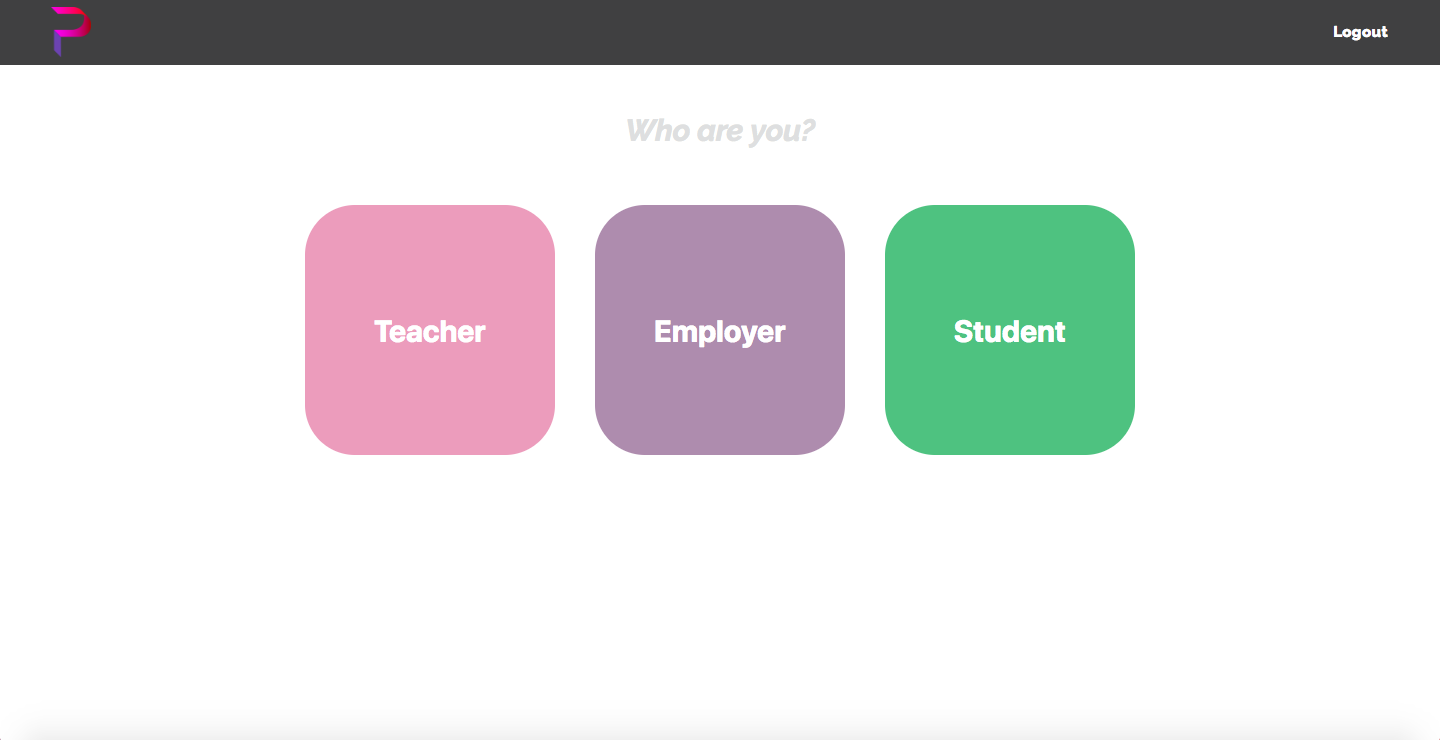
\includegraphics[scale=0.2]{type.png}
        \caption{Front-end view of what the user sees when beginning their PilotCity onboarding process. The user would then proceed accordingly, specifying what user category they would fall into.}
        \label{fig:usertype}
    \end{figure}

    \begin{figure}[H]
        \centering
        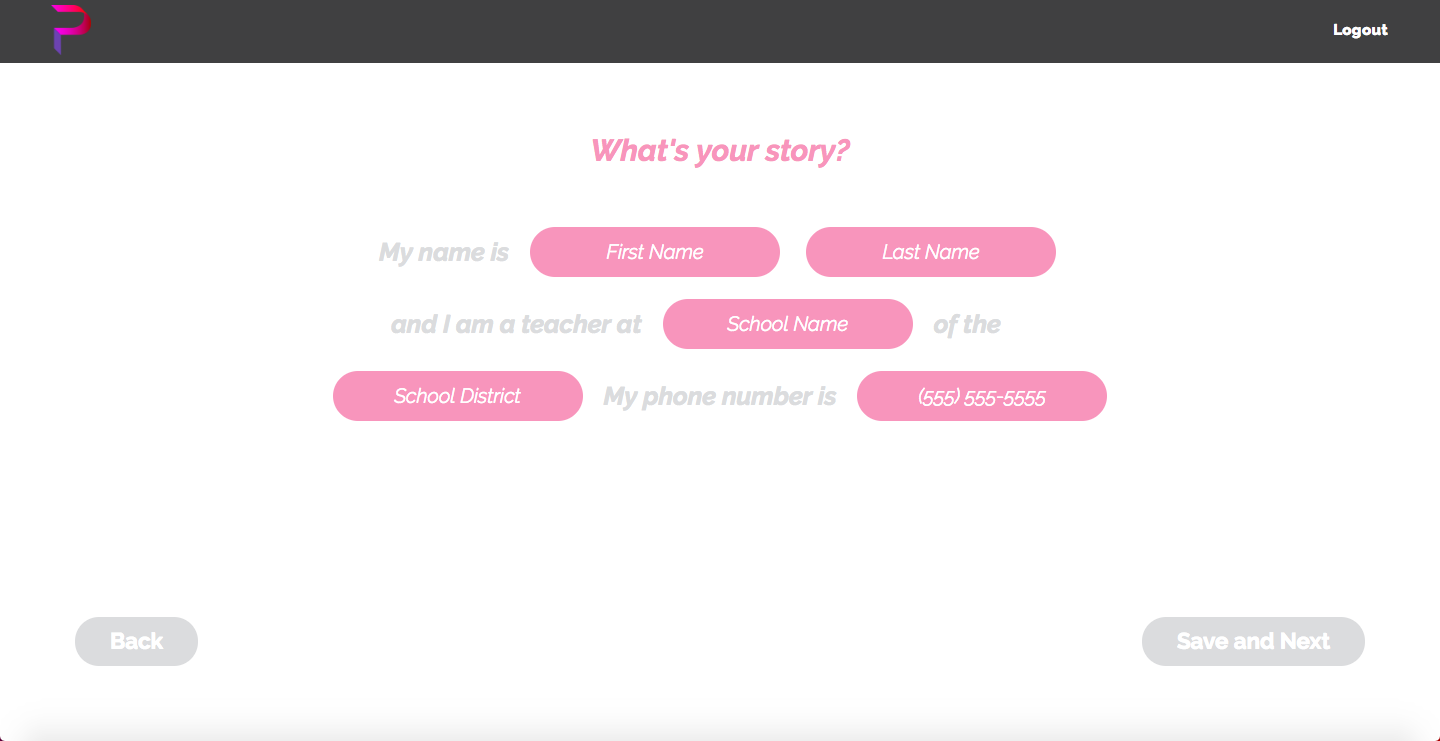
\includegraphics[scale=0.2]{story.png}
        \caption{The next page seen by an onboarding teacher. Here, the teacher is asked about the school they teach at and their contact information.}
        \label{fig:whatsurstory}
    \end{figure}
    
    \begin{figure}[H]
        \centering
        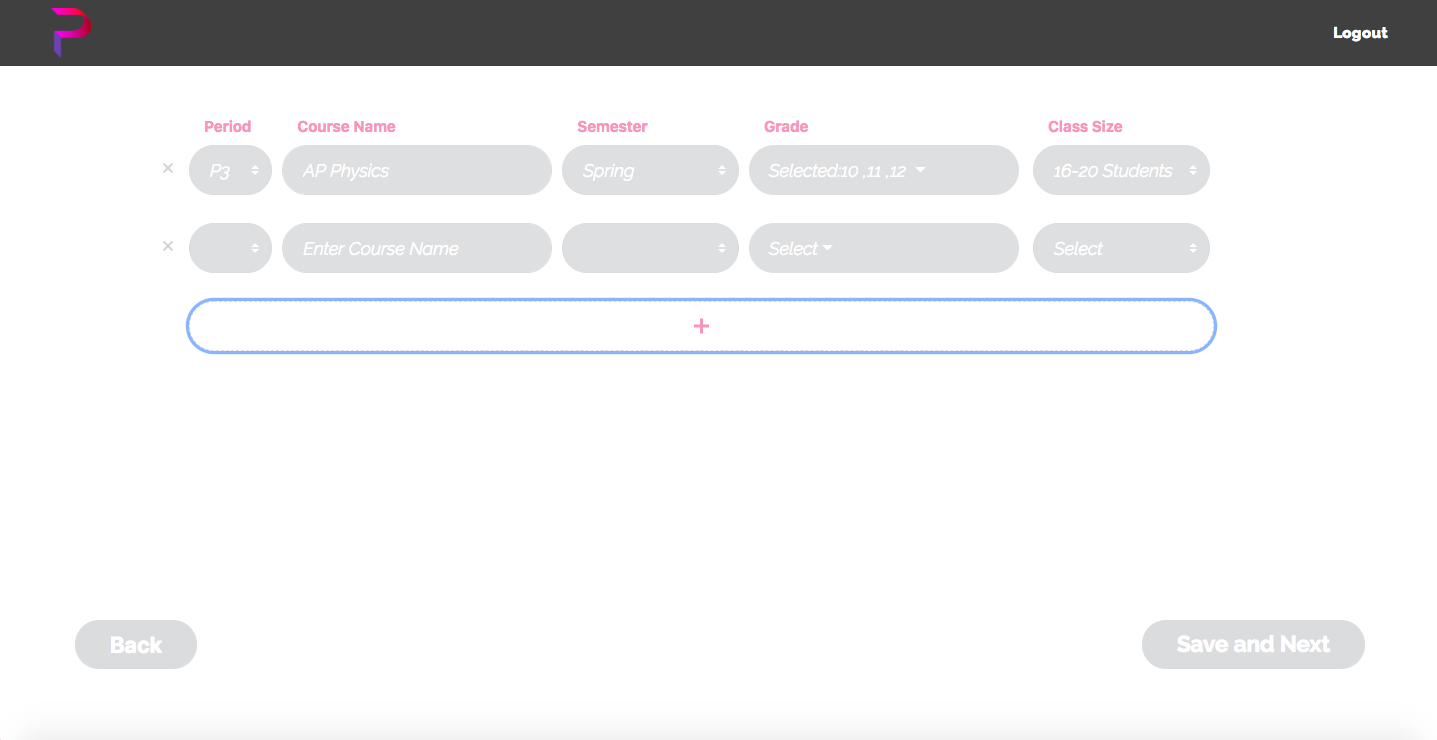
\includegraphics[scale=0.2]{classroom.png}
        \caption{Front-end view where the onboarding teacher is asked about the classes they want to involve in the PilotCity program.}
        \label{fig:describeclassroom}
    \end{figure}
    
    \begin{figure}[H]
        \centering
        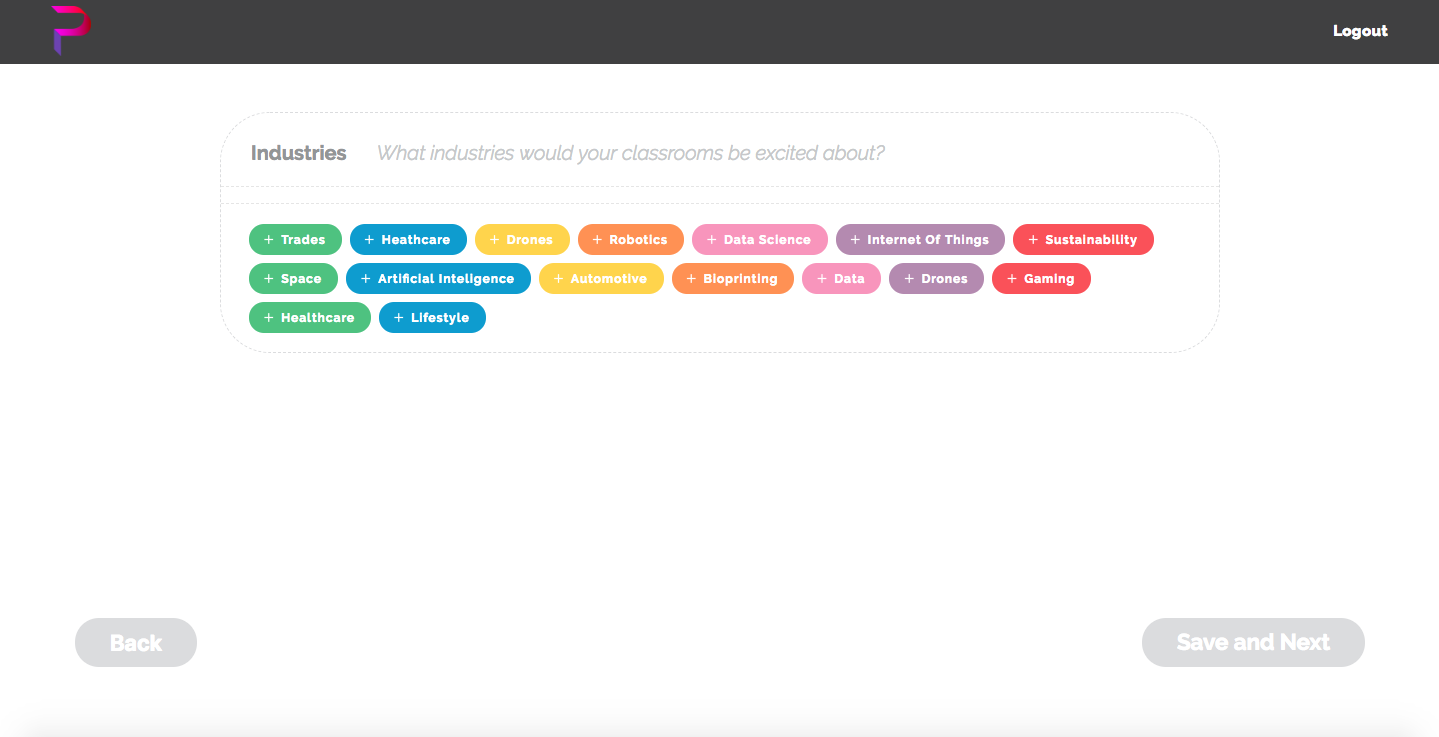
\includegraphics[scale=0.2]{industry.png}
        \caption{Front-end view where the onboarding teacher is asked about the industries that their classrooms would be interested in working with.}
        \label{fig:industrypref}
    \end{figure}
    
    \begin{figure}[H]
        \centering
        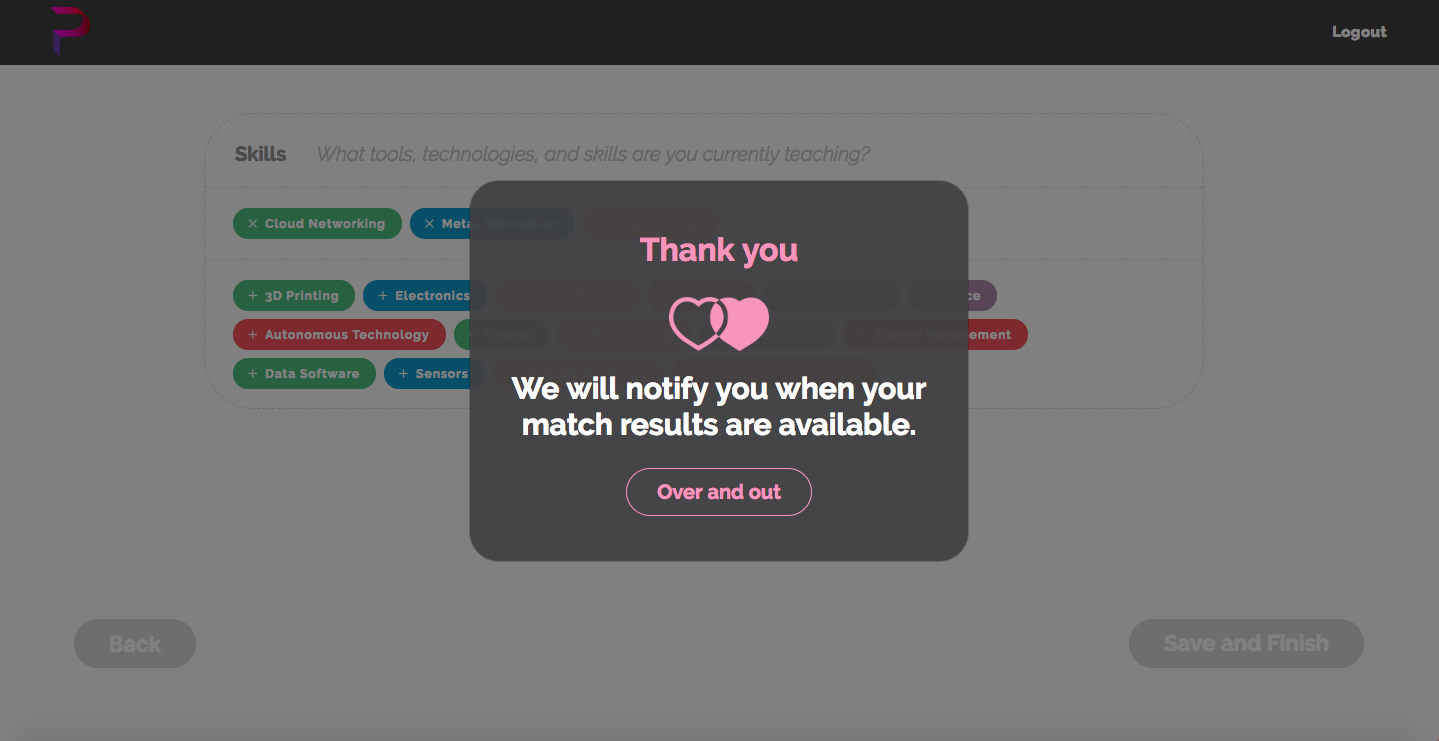
\includegraphics[scale=0.2]{end.png}
        \caption{View that the teacher would see once finishing the onboarding process. This page indicates to the user that their information has been saved, and that they will be contacted as soon as employer recommendations are available for each of their classrooms.}
        \label{fig:completed}
    \end{figure}

\subsection{Recommender System}

	We planned and implemented a recommender system to recommend classrooms to employers and employers to teachers based on similarities in industry and skills. We score classrooms for an employer and employers for a teacher using the GloVe Model, which represents words as vectors capturing semantic meaning. The similarity score between two words is taken to be the cosine of the angle between the vector representation of the two words. We further adapt the GloVe model's output to be able to take in two phrases with multiple words, such as "Machine Learning" and "Artificial Intelligence" and compute their similarity. This is done by taking the average of each pairwise similarity between individual words.
	
	The final score between an employer and a classroom is a weighted combination of the similarity scores between the inputs of employers and teachers. For each employer, we consider their industry, service, product, their vision for working with high school students, and the location of their workplace. For each classroom, we consider the course name, the industry preference of the teacher, the tools, technologies, and skills taught in the classroom, and the location of the school. The UI of the final recommendation system, as viewed by a logged in employer, is shown in figure \ref{fig:recommender_system} below. The final recommender system was meant to serve as a baseline ordering from which teachers and employers could easily choose suitable matches. 
	
	\begin{figure}[H]
        \centering
        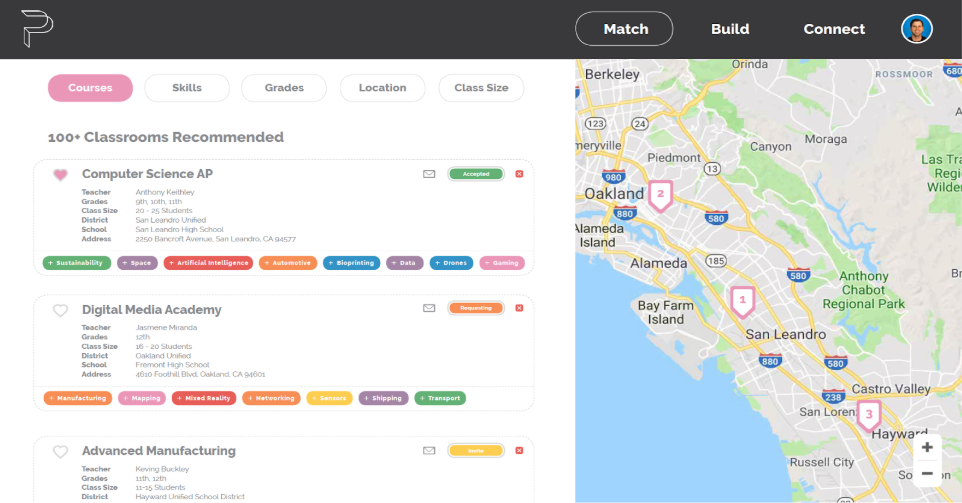
\includegraphics[scale=0.35]{recommender_ui.png}
        \caption{UI for the Recommender system}
        \label{fig:recommender_system}
    \end{figure}
	
\subsection{Evaluation of Recommender System}

The recommender system, due to a miscommunication between ourselves and the local team, was not correctly incorporated into PilotCity's website at the time of project placement which occurred over our winter break. For this reason, PilotCity made the final matches as they had done in previous years. We then evaluated our recommender system against the final project-placements in the following way. For each employer's assigned classrooms, we recorded what rank our recommender system gave each classroom. For example, one employer, the City of Hayward, was assigned 7 classrooms for spring 2019. Our recommender gave these 7 classrooms the ranks shown in the "our ranks" row in table \ref{tab:comp} below. We compare these ranks to what the "ideal ranks" would be (also shown table \ref{tab:comp}). Note that the lower the number, the more highly it is ranked (the classroom given a rank of 0 is the most highly-recommended classroom).

\begin{table}[H]
\begin{center}
\begin{tabular}{|l|l|l|l|l|l|l|l|l|l|l|l|l|l|l|}
\hline
\textbf{classroom}   & A  & B  & C  & D   & E & F & G  \\
\hline
\textbf{our ranks}   &  13 & 16 & 14 & 15 & 30 & 91 & 29  \\
\hline
\textbf{ideal ranks} & 0  & 1  & 2   & 3   & 4 & 5 & 6   \\
\hline
\end{tabular}
\end{center}
\caption{Comparison of classroom ranks for City of Hayward}
\label{tab:comp}
\end{table}


We can see from table \ref{tab:comp} above that our recommender, though imperfect, ranked the majority of the classrooms relatively high (13th, 14th, 15th, 16th place), yet some of the classrooms were ranked much deeper down the list, especially the outlier in 91st place. We create a score to encapsulate this trend.

Since all of the classrooms placed with the City of Hayward are equally suitable placements, any permutation of the ideal ranks is equally ideal. In order to account for this, our metric takes the median of our rank and compares that to the median of the ideal rank. We then subtract the median of the ideal rank from the median of our algorithm's rank to get a sense of how well, in aggregate, our recommender did for a given employer relative to that employer's ideal matching. For the above example with the City of Hayward, the score comes out to: 

$$ median(our\ ranks) - median(ideal\ ranks) = 16 - 3 = 13$$

Using the scoring method just described and averaging across all employers, our recommender system got a score of 34. Relative to over 150 total classrooms, this score is expected. Many of the variables that informed the final employer-classroom pairing decisions were factors we were advised to ignore to simplify the onboarding process, such as schedule and availability.

We considered tuning our recommender system's algorithm to minimize the score described above. However, we agree that at this stage with only 35 employers this approach would probably overfit our algorithm, especially as our score currently makes the strong assumption that each employer's "ideal" classrooms were the ones to which they were assigned. A more informative approach would be to gather data about how well classrooms and employers enjoyed their partnership and incorporate this into future recommender system iterations.

\subsection{Impact}

	A primary goal of our project has been to improve scalability, automation, and user engagement of PilotCity's efforts. 
	PilotCity having a website this year led to a major influx of new users. As PilotCity grows, they will be able to build off of our recommendation tool to optimize for the most successful classroom-employer partnerships. These improvements to PilotCity's programming may allow for more connections between high school students and workplace opportunities. These educational opportunities and general local connections benefit countless students and local cities which PilotCity serves. 

\subsection{Code}
    Our code is available on github.com/hmcmathclinic/18-19-PilotCity-Code and the most current version of the website can be viewed at pilotcity.com. 


%%% Chapter 4

%%% Copyright (C) 2004 Claire M. Connelly and 
%%% the Department of Mathematics, Harvey Mudd College.
%%%
%%% This file is part of the sample thesis document provided to HMC
%%% mathematics students.
%%%
%%% See the COPYING document, which should accompany this
%%% distribution, for information about distribution and modification
%%% of the document and its components.

\chapter{Extracting Insights From Text Data}%
\label{sec:figs-and-tabs}

Topic modeling is an unsupervised learning algorithm that takes in a large corpus of text data and returns a specified number of representative topics found in the corpus. A topic is defined as probability distribution over fixed vocabulary. Words in a topic are sorted in descending order using the probability assigned to each word in the topic. The top $k$ words in a topic (for some $k$ defined by the user) reflect the overarching and related concepts of the topic. Topic modeling therefore provides a method of extracting insights about the high level meaning of a text. 
An example of an output of topic modeling is shown in figure \ref{fig:distribution}.
\begin{figure}[H]
    \centering
    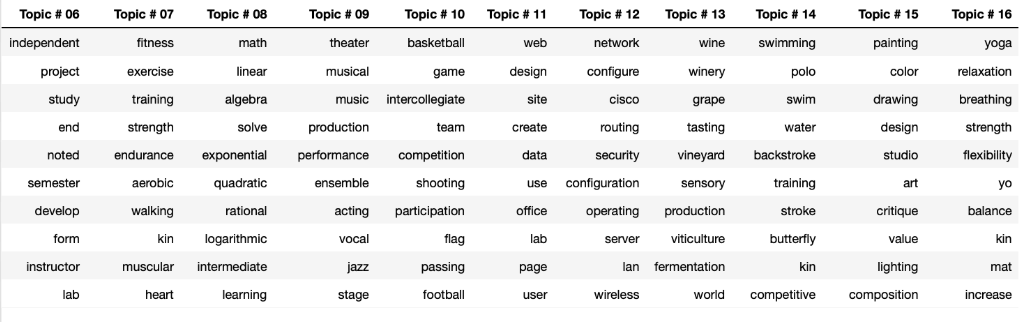
\includegraphics[scale=0.35]{topic-distribution.png}
    \caption{Example distribution of topics output by a trained topic model}
    \label{fig:distribution}
\end{figure}

\section{Methods}
Our team considered and explored two well-known methods for topic modeling:
    \begin{itemize}
        \item Latent Dirichlet Allocation, commonly known as LDA, is a generative probabilistic model that prescribes each document in a corpus with a finite mixture of topics from an underlying topic distribution. LDA views each document in a corpus as a generated item from a collection in order to infer the topic distribution. The generative process that LDA uses to infer the underlying topic distribution represents the topic distribution $\theta_m$ for each document $m$ as a random variable from a Dirichlet distribution with sparse priors, where each topic is a distribution over all of the words. For each of $N$ words in document $m$, a topic $z_n \sim \text{Multinomial}(\theta)$ is chosen and a word $w_n$ is chosen from a multinomial distribution conditioned on $z_n$. LDA requires the modeler to input number of topics. In our experiments, we built our LDA models from LdaModel in the gensim package. 

        \item Non-negative Matrix Factorization (NMF for short) takes in a bag-of-words $n\times m$ matrix $A$ whose entry $A_{ij}$ is the number of occurrences of word $j$ in document $i$. NMF seeks to find the closest approximation of $A$ as a product of a $n\times k$ matrix $W$ and a $k\times m$ matrix $H$ with the condition that all entries of $W$ and $H$ are non-negative. In other words, NMF outputs $W,H$ with the prescribed dimensions such that $\|A-WH\|_F$ is minimized.
        
        To interpret the output matrices $W$ and $H$, we call $W$ the \textit{basis matrix} and $H$ the \textit{coefficient matrix}. The prescribed number $k$ here represents the number of topics we wish to extract from the text. To find out the top words are associated with the $i$-th topic, we examine the $i$-th row of the $H$ matrix and take the words whose position in that row has a high value. In other words, the entry $H_{ij}$ measures how relevant word $j$ is for topic $i$. Next, if we want to find out what topics are the most prevalent in the $i$-th corpus document, we examine the $i$-th row of the $W$ matrix and take the topics whose position in that row has a high value. Although there are methods to perform this task with unseen documents that were not used in training, we omit their discussions here as they were not used for our experiments.
    \end{itemize}
In a later section, we discuss our preferred method and our reasons for choosing it.

\section{Assessing Insights}
\subsection{Topic Coherence}
Topic coherence is a standard method of comparing topic models. It measures how semantically cohesive each topic is. For example, we'd say that a topic that contained all medically-related words ("doctor," "stethoscope," "surgery," etc.) has a high coherence while a topic composed of unrelated words ("city", "toothpaste", "kittens") has low coherence. Our measure of coherence is the average pairwise similarity between the GloVe vector representations of the top three words of a given topic. 


By analyzing the mean topic coherence of a model compared to the number of topics in the model, we can determine the optimal number of topics for our model. As seen in figure \ref{fig:topic-coh}, topic coherence peaks where the model only has two topics. However, the team judged this to be an under-fit of the model. In this case, the optimal number of topics chosen was 16, the next highest peak. 
\begin{figure}[H]
    \centering
    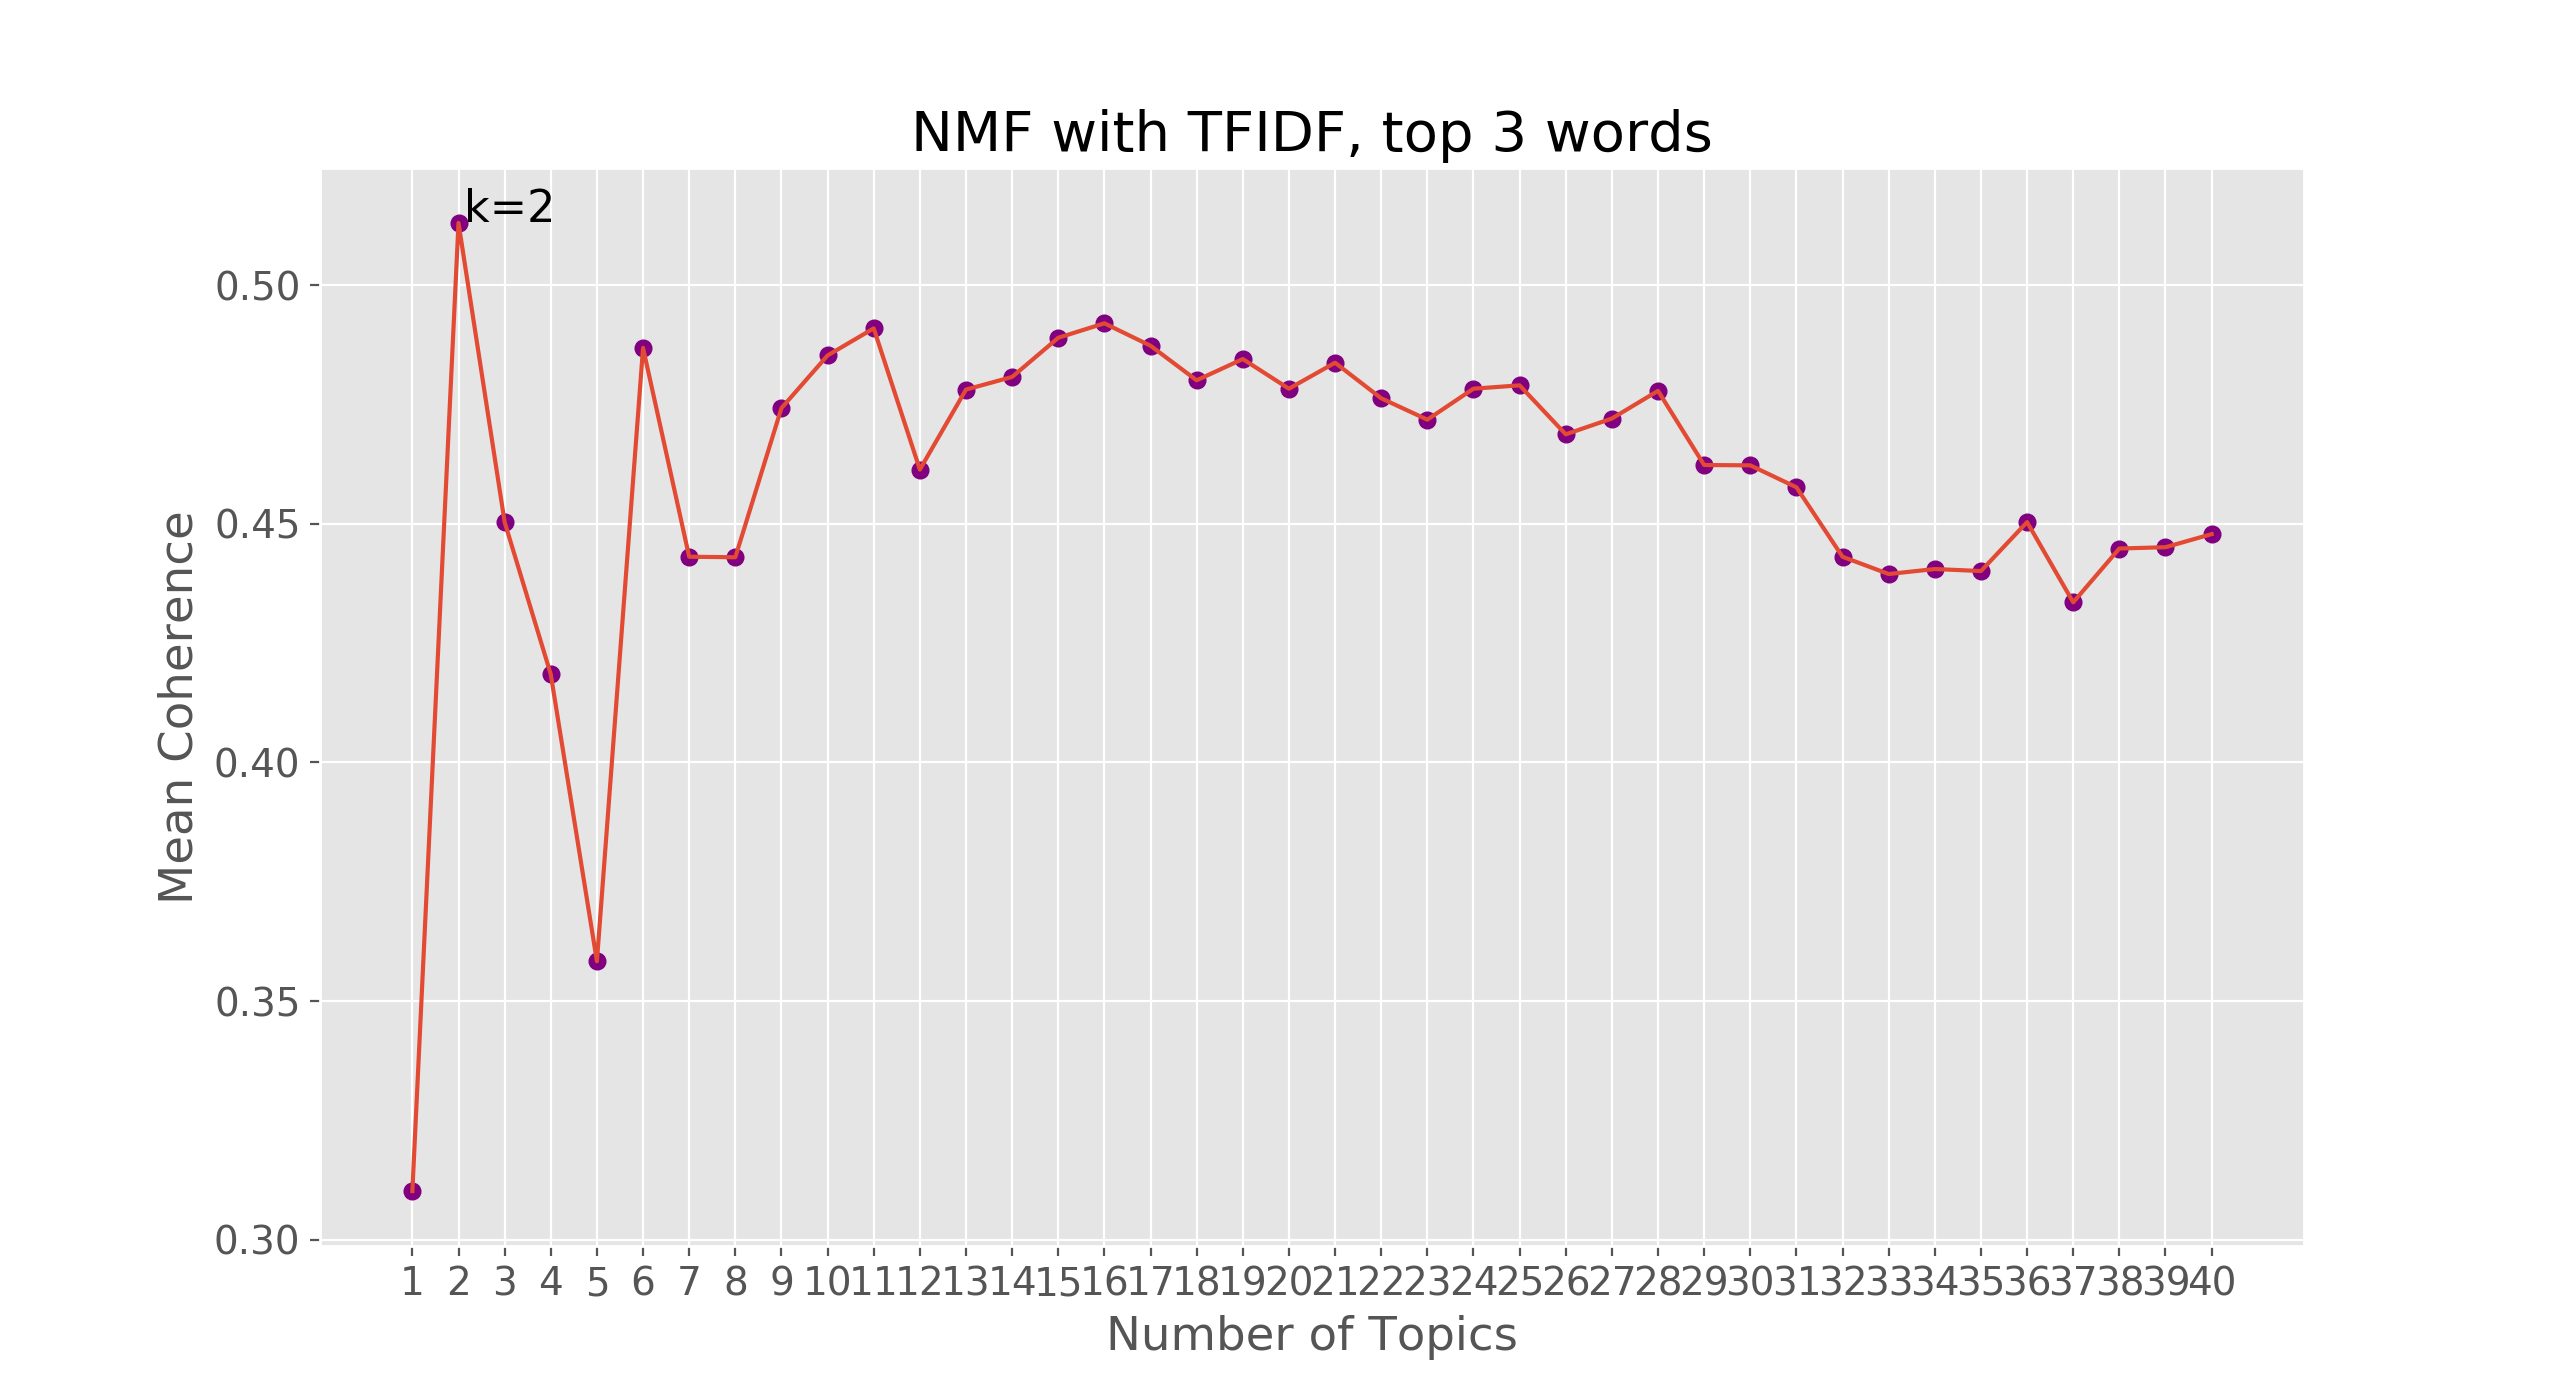
\includegraphics[scale=0.15]{topiccoh.png}
    \caption{Topic Coherence vs Number of topics using the first 3 words of every topic}
    \label{fig:topic-coh}
\end{figure}

\section{LDA vs NMF}
We ran experiments to determine which topic modeling technique would perform well for our purposes, specifically on Los Positas Syllabi. We trained models using both techniques and graphed the mean topic coherence of the outputs from the models to judge which technique performed better. From the graph in figure \ref{fig:lda_vs_nmf}, we see that for the range of number of topics considered, NMF consistently had higher mean topic coherence than LDA, and hence chose it for our model and the rest of our analysis. This was expected since NMF is said to perform better on sparser and smaller data sets (Chen, Zhang, Liu, Ye, \& Lin, 2019). However, we did provide flexibility in the module so that the modeler could use an LDA model if they prefer. 
\begin{figure}[H]
    \centering
    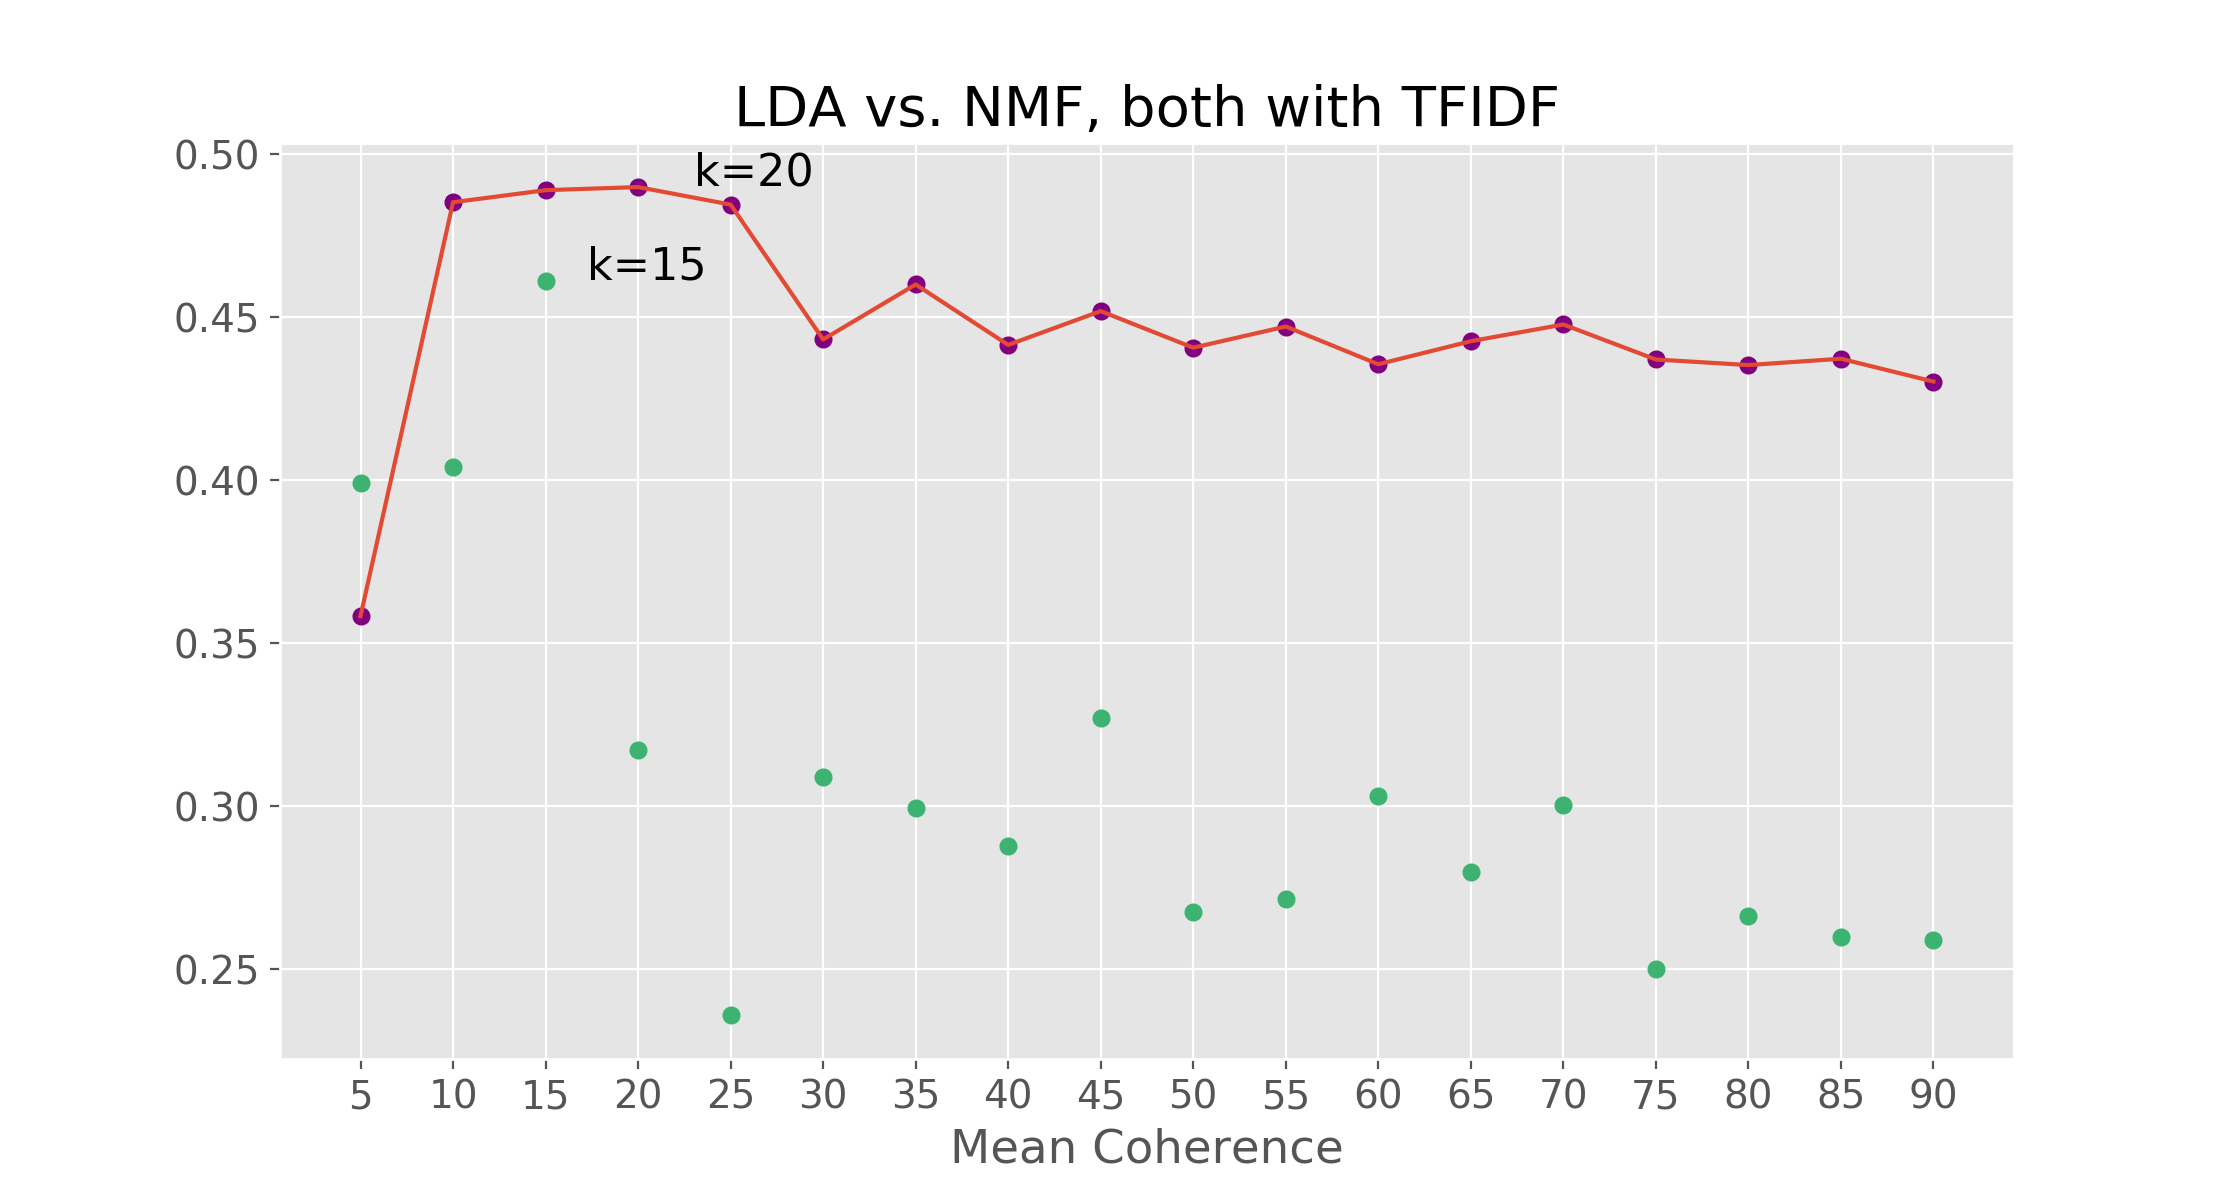
\includegraphics[scale=0.15]{LDAvsNMF.png}
    \caption{Topic Coherence of LDA compared to NMF. Models with NMF are shown with the line graph, and LDA are shown with dots}
    \label{fig:lda_vs_nmf}
\end{figure}

\section{Extracting insights}
Our goal is to leverage topic modeling to visualize high level themes represented in a corpus containing all the syllabi of an educational institution. By doing so, we can estimate the emphasis of each topic in the curriculum of the institution, as well as the overall educational priorities of the institution.

\subsection{Data}
Our dataset consists of 2,841 syllabi from Las Positas Community College in Livermore, California, which we obtained by scraping course syllabi publicly available on their \href{http://www.curricunet.com/laspositas/search/course/course_search_result.cfm}{website}.
\url{http://www.curricunet.com/laspositas/search/course/course_search_result.cfm}

\subsection{Visualization of Results}
The output of our trained NMF topic model is shown in figure \ref{fig:nmf-viz}. Each dot in this figure represents the 2D vector representation of a syllabus in the corpus. The color of these dots are determined by the topic they relate the most to. The top 3 words in each topic are printed alongside the syllabi-dots that are most related to it. Also, inter-dot distance is a measure of how similar the two syllabi are. 
\begin{figure}[H]
    \centering
    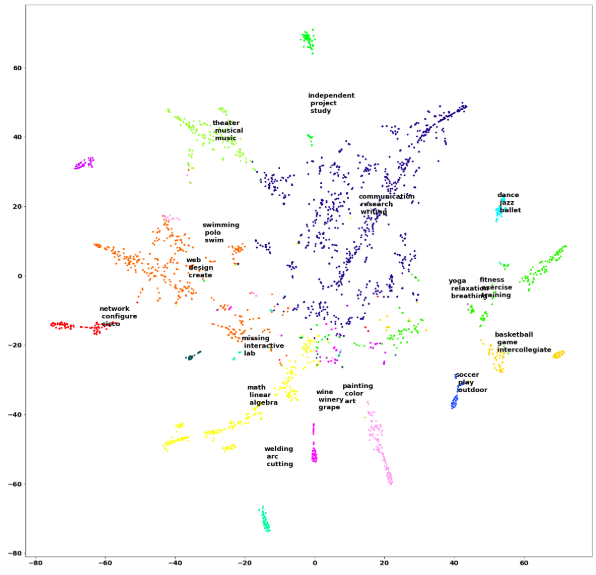
\includegraphics[scale=0.5]{nmf-visualization.png}
    \caption{Visualization of NMF results of Las Positas data. Here we see that the topic related to communication, research and writing is prevalent across many syllabi in the corpus. These syllabi-dots are also spread out, implying that the syllabi related to this topic are similar to other syllabi in the corpus as well. In contrast, the topic related to dance, jazz, and ballet is less prevalent, and is dominant in syllabi that are only similar to other syllabi within the same topic.}
    \label{fig:nmf-viz}
\end{figure}


\subsection{PilotCity Deliverable}

Our deliverable is a fully-functioning topic modeling package for PilotCity's use. The structure of our module is seen in figure \ref{fig:pipeline}. 
\begin{figure}[H]
    \centering
    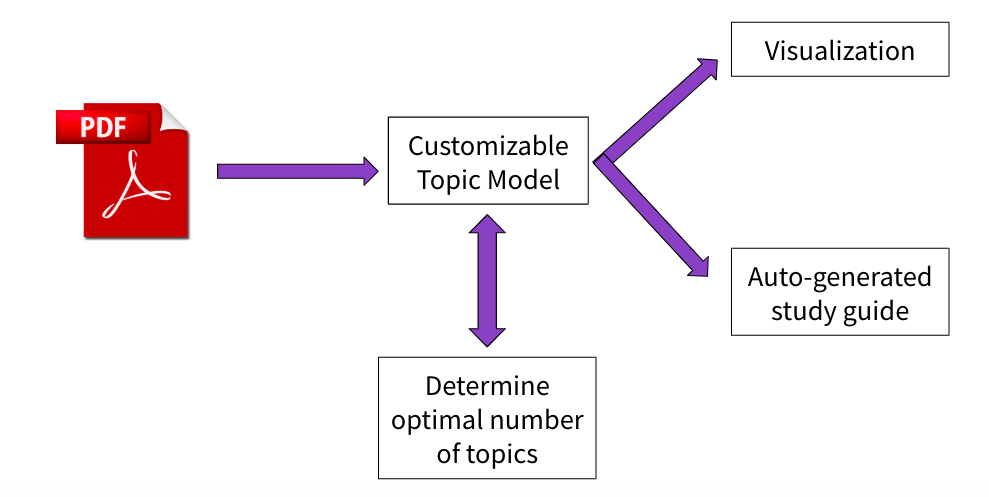
\includegraphics[scale=0.35]{module-pipeline.png}
    \caption{Pipeline for topic modeling module}
    \label{fig:pipeline}
\end{figure}
The module takes a folder of PDFs as input and cleans and tokenizes the text in each document. It also filters out the most common words across all documents using an algorithm called 'term frequency inverse data frequency', or TFIDF. These cleaned documents are used to train an NMF topic model, where the optimal number of topics is programmatically determined based on topic coherence. The model is saved, and visualized as in figure \ref{fig:nmf-viz}. 
Given an unseen syllabus and a trained topic model, our module can also extract the most representative topics from the syllabus and search Wikipedia for word definitions to automatically generate a study guide prototype. An example of an auto-generated study-guide is seen in figure \ref{fig:studyguide}.
We delivered the module to the PilotCity team and lead a training session to help them understand the potential use cases for the module during our spring site visit. 
\begin{figure}[H]
    \centering
    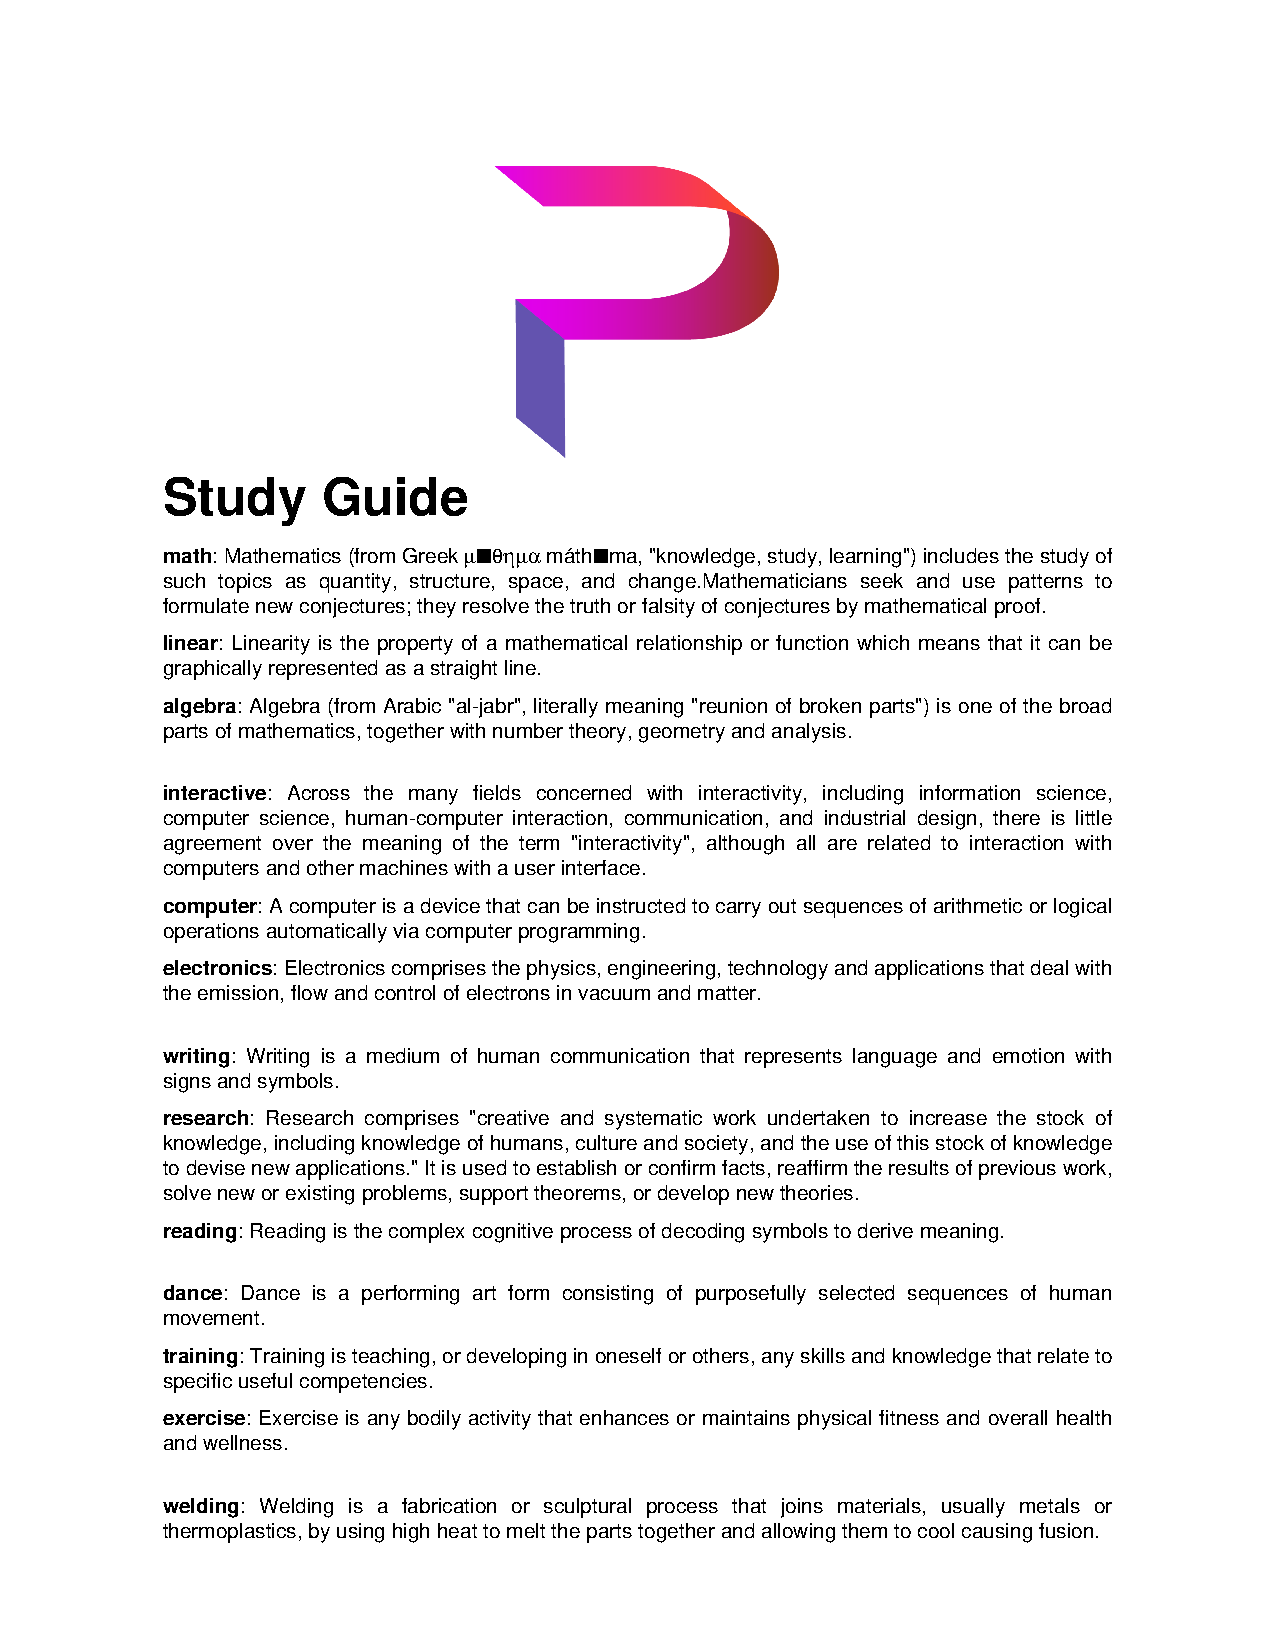
\includegraphics[scale = 0.5]{studyGuide_youJustMade.pdf}
    \caption{Auto-generated study guide}
    \label{fig:studyguide}
\end{figure}

\section{Further work with Topic Modeling}
In addition to running our topic model on syllabi of an institution to gauge current educational priorities, we also ran our topic model on syllabi of classes taught across many years to judge the change of an institution's educational priorities over time. This application is discussed further in the paper attached. 






%%% Chapter 5

%%% Copyright (C) 2004 Claire M. Connelly and 
%%% the Department of Mathematics, Harvey Mudd College.
%%%
%%% This file is part of the sample thesis document provided to HMC
%%% mathematics students.
%%%
%%% See the COPYING document, which should accompany this
%%% distribution, for information about distribution and modification
%%% of the document and its components.

\chapter{Conclusion}%
\label{sec:typesetting}

We conclude the year with the following accomplishments. We successfully built:

\begin{itemize}
    \item A launched website, created with the support of PilotCity's local team, which is already being used by PilotCity's academic and industry partners. 
    \item A maintainable, scalable Google Cloud database with secure log-in and optimized data structures.
    \item A recommendation engine to match classrooms and employers for projects. This engine: 
    \begin{itemize}
        \item harnesses Natural Language Processing tools like the GloVe model to place similarity scores on user inputs such as course names, industry preferences and project descriptions.
        \item outputs a ranked list of candidate classrooms/employers who are closely related. This list enables employers and teachers to easily discover each other for future partnerships.
    \end{itemize} 

    \item A module for visualization of educational priorities using topic modeling techniques. Features of this module include:
    \begin{itemize}
        \item Training a topic model on any collection of PDF documents. 
        \item Flexibility in the type of topic modelling techniques used. Currently, the module supports LDA and NMF. 
        \item Automated selection of optimal number of topics based on topic coherence.
        \item Visualizations of the topic distributions of an input PDF document. 
         
    \end{itemize}
    \item An engine that generates a guide for students which enumerates and defines the most important keywords contained in a classroom syllabus.  
\end{itemize}

Each stage of this project has been an iterative process involving multiple rounds of interviews and conversations with tech companies, school district administrators, high school teachers and other stakeholders to fully understand the impact of our work. From these interactions, our team has gained many insights about the educational system and the application of Natural Language Processing and automation to improve educational experiences.

%%% Local Variables: 
%%% mode: latex
%%% TeX-master: "master"
%%% End: 


%%% Chapter 6

%%% Copyright (C) 2004 Claire M. Connelly and 
%%% the Department of Mathematics, Harvey Mudd College.
%%%
%%% This file is part of the sample thesis document provided to HMC
%%% mathematics students.
%%%
%%% See the COPYING document, which should accompany this
%%% distribution, for information about distribution and modification
%%% of the document and its components.

\chapter{Future Work}%
\label{sec:figs-and-tabs}

\subsection{Improvements to Recommender System}

The current recommender algorithm requires that we specify weights to determine how much each input to the system contributes to a match result. This manual aspect of our algorithm could be removed by employing machine learning techniques to learn weights that lead to optimal matchings. This however would only be feasible after PilotCity has accumulated large enough employer-classroom matches and some measure of the success of the matchings. 

\subsection{Possible Extensions and Applications of Insights Engine}
This report detailed how we investigated the potential to extract insights in the form of topic distributions from syllabi. This idea could be used by PilotCity to assist in the onboarding process where teachers have to supply keywords that describe the classrooms they teach. That is, PilotCity can have teachers upload course syllabus for a specific classroom and our trained insights engine would generate the top keywords that describe the nature of the class rather than having the teacher manually fill out this information.
\newline

One application of our insights engine that we explored in the report was the generation of a guide with definitions of overarching topics pertaining to a syllabus. We could improve these automatically generated guides to provide more contextualized information by performing network analysis on Wikipedia's clickstream data to gain insights on what pages people visit right before and right after going to the Wikipedia page pertaining to a topic.

%%% Local Variables: 
%%% mode: latex
%%% TeX-master: "master"
%%% TeX-master: "master"
%%% End: 



%%% Back matter.

%%% The back matter of a document is where the bibliography and index
%%% are defined.  It starts, not surprisingly, with the \backmatter
%%% command. 

\backmatter


%%% Bibliography.

%%% BibTeX is the tool to use for citations and layout of your
%%% bibliography.  Instead of having to type ``[5]'' or ``(Jones,
%%% 1968)'' (and keep track of which citation is which and renumber
%%% them as you add more references to your bibilography), you use
%%% special commands that allow BibTeX and LaTeX to automatically put
%%% the correct information in the right place.

%%% Depending on your field, it may or may not be appropriate to list
%%% references for which you haven't included specific citations.  If
%%% your field sanctions such practices, or if you just want to get an
%%% idea of what you have in your bibliography file, you can include
%%% everything with the \nocite{*} command.
% \nocite{*} 


%%% The appearance of your bibliography and citations in your text are
%%% defined by a combination of any bibliography-related LaTeX
%%% packages (such as natbib, harvard, or chicago) and the particular
%%% bibliography style file that you load with the \bibliographystyle
%%% command.  Bibliography-style files end in .bst; you can find them
%%% by searching your file system using whatever tools you have for
%%% doing searches.  (On most modern Unices, ``locate .bst'' will give
%%% you an idea of what's available.)

% \bibliographystyle{plainnat}

%%% The particular bibliography data file or files that you want to
%%% use are specified with the \bibliography file.  Multiple files are
%%% separated by commas.

%%% You might want to use multiple bibliography (or ``bib'') files if
%%% you had a master bib file containing references you use again and
%%% again, and another containing only records for references for a
%%% particular project.

%%% Many people create a single, large bib file that they use for
%%% everything they write.  That approach requires you to \cite every
%%% reference that you want to use in your document -- using
%%% \nocite{*} with a huge bibliography database will give you a large
%%% bibliography containing many references you haven't consulted for
%%% your particular document!
\bibliographystyle{apacite}
% \bibliographystyle{plain}

\bibliography{bibliography}
\nocite{*}

%%% Glossary or Index.

%%% If you were going to include a glossary or index in your document,
%%% the relevant commands would appear here.

%%% If you think that you would like to include such features, talk
%%% with someone who's worked with LaTeX a lot very early in your
%%% writing process.  These commands require you to do a bit of
%%% thinking about what you would want to index or gloss in advance --
%%% going back though a completed document to add \index commands is
%%% *not fun*.

\end{document}


